	\documentclass[twoside]{article}
\usepackage{../../estilo-ejercicios}

%--------------------------------------------------------
\begin{document}

\title{Ejercicios de Topología Algebraica}
\author{Javier Aguilar Martín}
\maketitle

\begin{ejercicio}{1}
Probar que para todo $p\geq 0$ se tiene 
\[
C_p(K;\Z)\cong Z_p(K;\Z)\bigoplus B_{p-1}(K;\Z)
\]
y deducir 
\[
C_p(K;\Z)/B_p(K;\Z)\cong H_p(K;\Z)\bigoplus B_{p-1}(K;\Z)
\]
\end{ejercicio}
\begin{solucion}
Tenemos la sucesión exacta corta
\[
0\to Z_p(K;\Z)\hookrightarrow C_p(K;\Z)\xrightarrow{d_p} B_{p-1}(K;\Z)\to 0.
\]
Todos los grupos que aparecen son libres abelianos, bien por definición en el caso de $C_p(K;\Z)$, bien por ser subgrupos de un grupo libre abeliano en los otros dos casos. Por tanto, esta sucesión exacta corta escinde (para grupos libres abelianos se demuestra de forma idéntica al caso de espacios vectoriales). Así que concluimos que 
\[
C_p(K;\Z)\cong Z_p(K;\Z)\bigoplus B_{p-1}(K;\Z).
\]
PREGUNTAR SI TENGO QUE DEMOSTRAR LO DE QUE SUBGRUPO DE LIBRE ABELIANO ES LIBRE ABELIANO

Ahora, como $B_p(K;\Z)$ es un subgrupo de $Z_p(K;\Z)$, al hacer el cociente deducimos
\[
C_p(K;\Z)/B_p(K;\Z)\cong Z_p(K;\Z)/B_p(K;\Z)\bigoplus B_{p-1}(K;\Z)=H_p(K;\Z)\bigoplus B_{p-1}(K;\Z).
\]
\end{solucion}

\newpage

\begin{ejercicio}{2}
Calcula los grupos de homología simplicial del complejo siguiente
\begin{figure}[h!]
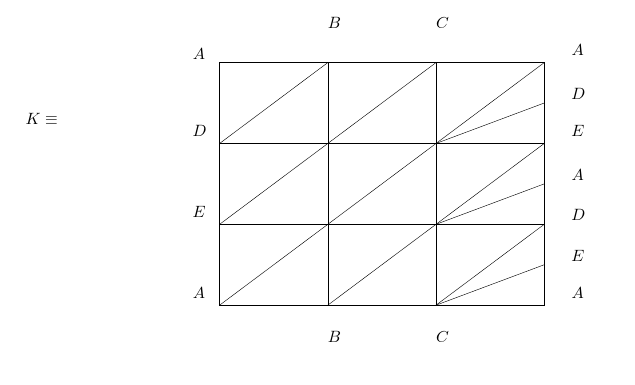
\includegraphics[scale=0.8]{K}
\end{figure}
\end{ejercicio}
\end{document}
